\documentclass{article}
\usepackage{zpj}
\usepackage{tikz}
\newcommand{\comm}[1]{\ {\color{blue} \texttt{#1}}\ }
\begin{document}
\zihao{-4}
\title{计算物理(B)上机实验报告}
\author{朱沛俊\\ PB12203216\\近代物理系}
\maketitle
\section{有限差分法}
由于题目的边界十分规则,因此采用有限差分法计算起来十分简单,只需要利用公式:
\[\varphi_{i,j}=(\varphi_{i-1,j}+\varphi_{i+1,j}+\varphi_{i,j-1}+\varphi_{i,j+1})/4\]
不断进行迭代即可。

本程序\comm{yxcf.py}是用python语言写的,采用松弛因子$\omega=2/(1+\sin(\pi/n))$的超松驰迭代。直接运行它会得到默认的分割对应的的结果。也可以在python3中import它,然后调用相关函数。具体函数用法可以参见注释或者导入模块后用\comm{help()}命令。函数说明:
\begin{itemize}
 \item \comm{gridcf()}采用$n\times n$的分割以及默认的边值函数,迭代计算$\varphi$的值
 \item \comm{sid()}函数是边值函数
 \item \comm{yxcf()}采用$n\times n$的分割,迭代计算$\varphi$的值。需要输入边值函数。
 \item \comm{print3()}按三位有效数字打印数组
\end{itemize}
\section{有限元素法}
用有限元素法解Laplace方程第一边值问题,就是利用了能量最低原理,系统的能量
\[E\propto \int(\nabla\varphi)^2\dd S\]
其中$\propto$符号表示正比于。下面采取了与书上不同的一个推导,得出了一个形式紧凑的公式\ref{comp}。
\subsection{三角形域的能量公式推导}
对于某个三角形$ABC$而言,假设它的三个点电势分别为$\varphi_a,\varphi_b,\varphi_c$。如图\ref{nab}所示,取$AB'\perp AC, AC'\perp AB$,则将$\nabla\varphi$的分量合成,有:
\[(\nabla\varphi)^2=\frac{1}{\sin^2 A}\left(\frac{\varphi_{ab}^2}{c^2}+\frac{\varphi_{ac}^2}{b^2}-\frac{2\varphi_{ab}\varphi_{ac}\cos A}{bc}\right)\]
\begin{figure}[htbp]
\centering
 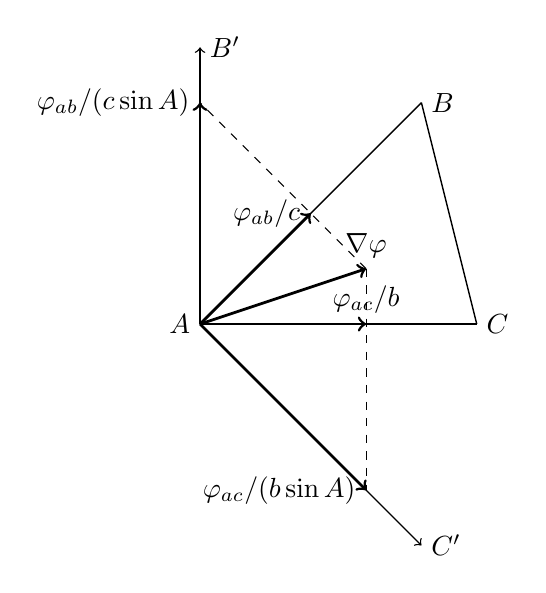
\begin{tikzpicture}
\pgfsetxvec{\pgfpoint{20pt}{0}}
\pgfsetyvec{\pgfpoint{0}{20pt}}
  \draw[->,line width=0.5pt] (0,0)node[left]{$A$}--(4,-4)node[right]{$C'$};
  \draw[line width=0.5pt] (0,0)--(5,0)node[right]{$C$};
  \draw[line width=0.5pt] (4,4)node[right]{$B$}--(5,0);
  \draw[line width=0.5pt] (0,0)--(4,4);
  \draw[->,line width=0.5pt] (0,0)--(0,5)node[right]{$B'$};
  \draw[dashed] (3,1)--(0,4);
  \draw[dashed] (3,1)--(3,-3);
  \draw[->,line width=1pt] (0,0)--(2,2)node[left]{$\varphi_{ab}/c$};
  \draw[->,line width=1pt] (0,0)--(3,-3)node[left]{$\varphi_{ac}/(b\sin A)$};
  \draw[->,line width=1pt] (0,0)--(0,4)node[left]{$\varphi_{ab}/(c\sin A)$};
  \draw[->,line width=1pt] (0,0)--(3,0)node[above]{$\varphi_{ac}/b$};
  \draw[->,line width=1pt] (0,0)--(3,1)node[above]{$\nabla\varphi$};
 \end{tikzpicture}
 \caption{用协变与逆变基求解$(\nabla\varphi)^2$}\label{nab}
\end{figure}

而它的面积满足:
\[S=\frac{bc\sin A}{2}\]
三角形内的能量满足:
\begin{align}
 E_{\triangle}&\propto S(\nabla\varphi)^2\\
 &\propto \frac{bc}{\sin A}\left(\frac{\varphi_{ab}^2}{c^2}+\frac{\varphi_{ac}^2}{b^2}-\frac{2\varphi_{ab}\varphi_{ac}\cos A}{bc}\right)
\end{align}
对$\varphi_a$求导得到:
\begin{equation}
 \frac{\pp E_\triangle}{\pp \varphi_a}\propto \left(\frac{b}{c\sin A}-\cot A\right)\varphi_{ab}+\left(\frac{c}{b\sin A}-\cot A\right)\varphi_{ac}\label{a}
\end{equation}
其中:
\[\frac{b}{c\sin A}-\cot A=\frac{b-c\cos A}{c\sin A}=\frac{a\cos C}{a\sin C}=\cot C\]
同理\[\frac{c}{b\sin A}-\cot A=\cot B\]
故\ref{a}化为
\begin{equation}
 \frac{\pp E_\triangle}{\pp \varphi_a}\propto \varphi_{ab}\cot C+\varphi_{ac}\cot B
 \label{comp}
\end{equation}
\subsection{能量取极值时电势的驻点方程}
设$E$为总能量,用$i$标记所有包含$A$点的三角形,$B_i, C_i$对应于三角形$i$中的另外两个顶点,则:
\begin{align}
 \frac{\pp E}{\pp \varphi_a}&=\sum_i\frac{\pp  E_i}{\pp \varphi_a}\\
 &=\sum_i \varphi_{ab_i}\cot C_i+\varphi_{ac_i}\cot B_i
\end{align}
总能量取极值时,对所有的内点$A$满足$\pp E/\pp \varphi_a=0$时,:
\[\sum_i \varphi_{ab_i}\cot C_i+\varphi_{ac_i}\cot B_i=0\]
\[\left(\sum_i\cot C_i+\cot B_i\right)\varphi_{a}=\sum_i \varphi_{b_i}\cot C_i+\varphi_{c_i}\cot B_i\]
最终得到:
\[\varphi_a=\frac{\sum_i \varphi_{b_i}\cot C_i+\varphi_{c_i}\cot B_i}{\sum_i\cot C_i+\cot B_i}
\]

遍历所有的内点,用此方程进行迭代求解就可以求得区域内势函数$\varphi(x,y)$的近似解。
\subsection{三角形各角的余切值的计算}
假设给定了三个点$A,B,C$的坐标$(x_i,y_i)$(计算叉乘时取坐标$z_i=0$),设$\bm b=\bm{AB}, \bm c=\bm{AC}$则
\begin{align}
 \cot A&=\frac{bc\cos A}{bc\sin A}\\
       &=\frac{\bm{b\cdot c}}{|\bm{b\times c}|}\\
       &=\frac{\bm{b\cdot c}}{2S}
\end{align}
显然分子分母都是易于计算的形式,且分母对于三个角都是一样的,故只需要计算一次即可。
用这个公式也可以类似地计算出系数$\cot B_i$和$\cot C_i$。
\subsection{程序的具体实现}
本程序\comm{yxys.py}用python语言写成,调用了它的scipy库里面的稀疏矩阵类。直接运行会得到默认分割方式的结果,它的分割方法是先像有限差分法那样分割,然后再把每个小正方形从左上角到右下角分割为两个三角形。也可以在python3中import它,然后调用相关函数。具体函数用法可以参见注释或者导入模块后用\comm{help()}命令。函数说明:
\begin{itemize}
 \item \comm{gridtri()}函数会给出一类分割,可以调节分割的精细程度$n$
 \item \comm{yxys()}函数可以对任意的分割方式给出有限元素法的迭代解,返回值为所有节点的$\varphi$值。
 \item \comm{tris()}产生了一个特定的三角形分割
 \item \comm{points()}和\comm{sdp()}分别产生了相应于该分割的内点与边界点的点列
 \item \comm{tricot()}函数负责计算三个点对应的$\cot \theta_i$
\end{itemize}
\end{document}
